This chapter presents an overview of the main works focused on the topics addressed in this dissertation.

\section{Related Works Description}
\label{s:RelatedWorks-Description}

The state-of-the-art presents different computational techniques for data analysis. Lots of works found in the \ac{WWT} field use a combination of them to achieve their goal and improve the operation of the \acs{WWTP}s. Most works aim to accomplish fault detection, control, soft-sensing, variable prediction, or process understanding, among others. Special attention will be given to the prediction task since it is the main focus of this investigation.
%either physical modelling, can have different purposes,

\ac{WWTP}s are systems that exhibit a complex dynamic and require high performance to accomplish the standards imposed by the environmental regulatory authorities \cite{Corominas2018}. Considering the complex process nature, which presents a nonlinear behaviour and involves the interaction of physical, chemical, and biological components, it becomes crucial to estimate and predict key process variables. These variable predictions enhance the control, process monitoring and simulation that increase the efficiency of the treatment and the quality of the effluent \cite{Aalami2019,Arismendy2020,Liu2020}. Artificial intelligence methods are commonly used for solving the estimation and prediction challenges in nonlinear engineering science problems \cite{Lotfi2019}. Literature introduces a wide landscape of strategies and techniques to achieve the mentioned task. \autoref{f:Techniques-Distribution} \cite{Corominas2018} shows the distribution of computational techniques used in the field of wastewater treatment for fault detection, prediction, soft-sensing, process understanding, control and optimization, among others, it is made based on the number of papers published and cited in recent years. 

\begin{figure}[t]
\centering
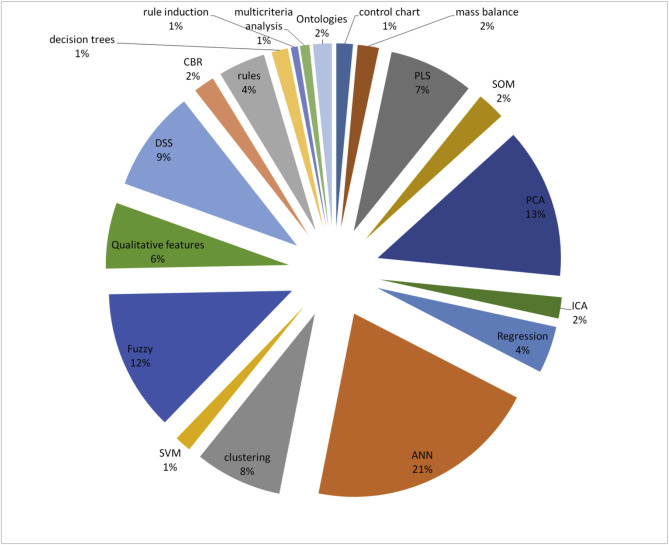
\includegraphics[width=15cm]{figures/3-Distribution-of-papers.jpg}
\caption{Techniques distribution \cite{Corominas2018}.}
\label{f:Techniques-Distribution}
\end{figure}

Research carried out by \cite{Corominas2018} shows that most of the papers published use \ac{ANN}, \ac{PCA} and \ac{FL} which are present in 46\% of the papers studied. Regarding the prediction tasks, which is the focus of this work, \ac{MLR} models, \ac{FL}, \ac{PLS}, \ac{ANN} and \ac{SVM} are the main methods used, where the last two stand out on nonlinear supervised learning. Other techniques involved in prediction are \ac{PCA}, Self-organizing Maps \ac{SOM}, clustering, and Qualitative features commonly used for dimensionality reduction, information extraction, problem understanding, and variable selection.

One of the early approximations to intelligent monitoring and the predicting system was presented in \cite{Sanguesa2000}, and \cite{Haggege2005}, where Bayesian networks and neuro-fuzzy logic were implemented to fulfil limitations of rule-based systems. Further works started to focus their attention on variable prediction using various methods and a combination of them, taking the major advantages offered by each one. Reference \cite{Qin2012} used iterative predictor weighting–partial least squares boosted by weighted predictions of a collection of regression models used as an ensemble prediction to estimate some water quality parameters. It was tested in the field, and its results showed a high correlation of the prediction. 

Several recent studies used fuzzy logic or neuro-fuzzy systems, such as \cite{Nourani2018,Nadiri2018,Han2018}, and some deep learning approaches, as in \cite{Guo2015,Alsina2018,Dairi2019}, which have provided high performance in prediction tasks. Studies like \cite{Bagheri2015} used a hybrid artificial neural network–genetic algorithm approach to optimize the \ac{ANN} estimation of the sludge bulking present in the sedimentation stage, which directly affects the effluent discharge water quality. Reference \cite{Dellana2009} made a performance comparison between the \ac{ARIMA} and time-delay neural network \ac{TDNN} with such times-series variables as \ac{BOD} and \ac{TSS} and achieved more accurate predictions for real-world wastewater data with \ac{TDNN}.

\section{Variable Prediction}
\label{s:RelatedWorks-variablePrediction}

\cite{Zhou2019} proposes a set of decision-tree regression models to predict daily wastewater influent in two \ac{WWTP}s located in Ontario. Results for training and testing exhibit a \begin{math}R^2\end{math} of 0.97 and 0.72 for one facility and the second one 0.96 and 0.58, respectively. \cite{Lu2020} evaluates the performance of two decision-tree-based ensemble learners and enhances their performance with a data denoising technique called \ac{CEEMDAN} to predict Temperature, Dissolved Oxygen, pH, Specific Conductance, and fluorescent dissolved organic matter. The enhanced Extreme Gradient Boosting and \ac{RF} show the best results among other techniques used in the experiments, obtaining \ac{MAPE}s from 0.27\% to 14.94\% in the best cases, depending on the variable selected to predict.

Study \cite{Alsulaili2021} implements a \ac{FFNN} to predict the effluent \ac{BOD}, \ac{COD} and \ac{TSS} in Kabd \ac{WWTP}, Kuwait. The authors train the model with 1032 samples and take as input different influent parameters. This work presents a \begin{math}R^2\end{math} score of 0.75, 0.61 and 0.63, respectively. Also, \cite{Abba2017} determines the efficiency of \ac{ANN} in predicting effluent \ac{COD} of Nicosia \ac{WWTP}, Chipre. Six different \ac{ANN} models are trained where diverse model structures, input variables and epochs of training are considered. The best results obtained present a \begin{math}R^2\end{math} of 0.70 which is an improvement compared with the baseline they established using \ac{MLR} and obtained \begin{math}R^2\end{math} of 0.34.

Work \cite{Niu2020} proposes a hybrid predictive model that uses \ac{DBN}, a  structure specialized in regression tasks. A \ac{GA} optimizes the hyperparameters of the network achieving a \ac{MAPE} of 4.34\% and \begin{math}R^2\end{math} of 0.6 for the effluent \ac{COD} prediction.

Reference \cite{Zhao2021} compares the impact of the optimization algorithm used during the training of a \ac{FFNN} implemented with the aim of predicting effluent \ac{TN}. The baseline model uses backpropagation optimization algorithm and achieves a \begin{math}R^2\end{math} value of 0.85 and 0.26 for training (104 data points) and testing dataset (20 data points), respectively. The implementation of \ac{L-M}, \ac{BR}, and Scaled Conjugate Gradient optimization algorithms shows an improvement in the overfitting of the baseline model, obtaining \begin{math}R^2\end{math} of 0.88, 0.84, and 0.84 during training and 0.87, 0.78, and 0.86 over the whole set respectively.

Another example \cite{Manu2017} compares the performance of  \ac{SVM}s and \ac{ANFIS} in the prediction of discharge \ac{TN} concentration for the Kavoor \ac{WWTP} located at Mangalore. \ac{ANFIS} are fuzzy logic systems where the structure is replaced by a neural network. Experiments show that \ac{SVM}s overcome the results obtained by the \ac{ANFIS}, achieving a \begin{math}R^2\end{math} of 0.82 versus 0.62 with Trapezoid Membership Functions and 0.72 with Gaussian Membership Functions. 

Work \cite{Guo2015} aims to predict one-day interval \ac{TN} concentration of effluent stream from Yong-yeon \ac{WWTP} in Ulsan, Korea. Measurements of some parameters from different points of the treatment serve as inputs for two \ac{ML} models: \ac{ANN} and \ac{SVM}. Results show a \begin{math}R^2\end{math} for training and validation of 0.55 and 0.47 for the \ac{ANN} and 1.00 and 0.46 for the \ac{SVM} approach. Both models use 200 and 90 samples for training and validation process, respectively.

Recurrent neural networks are also used in wastewater data-driven modelling. \cite{Yaqub2020} uses \ac{LSTM} Neural Networks to predict removal efficiency of NH4-N, \ac{TN}, and \ac{TP} from a \ac{WWTP} at Okcheon, Republic of Korea. A year of data with hourly frequency measurements constitutes the dataset used for this work. A set of 5000 data points build the sequences of 10 previous observations used to train the  \ac{LSTM} model. The testing step shows the \ac{MSE} values of 0.0047, 0.015, and 0.018, respectively, by using 1876 new data points. Study \cite{Kang2020} proposes a \ac{LSTM} and compares the results with \ac{SVM}, \ac{GRU} Neural Network, and standard  \ac{Bi-LSTM}. Experiments show that \ac{Bi-LSTM} performs at least as well as other models and obtain better results in some scenarios.

A \ac{GRNN} is implemented in \cite{Heddam2016}, a network architecture made of four layers: the input layer, the pattern layer, the summation layer, and the output one. This architecture offers high performance in non-linear regression analysis, the reason why it is used to estimate the effluent \ac{BOD} based on other effluent parameters. Results are compared with a \ac{MLR} showing that the \ac{GRNN} performs better for the \ac{BOD} estimation, achieving \begin{math}R^2\end{math} of 0.75 and 0.80 for training and testing, where 553 and 138 samples are respectively used. 

\cite{Baki2019} test the predictive capabilities of diverse regression models used to estimate the \ac{BOD} in the Antalya Hurma \ac{WWTP}. The study implements four different methods; classical regression analysis, Multivariate Adaptive Regression Splines, Artificial Bee Colony, and teaching learning-based optimization. \cite{Baki2019} uses 186 samples corresponding to 80\% of the available data to train all four proposed techniques, which yield \begin{math}R^2\end{math} values of 0.74, 0.79, 0.78, and 0.74 over the test dataset.

\cite{Guo2020} innovates in the use of \ac{CNN} together with \ac{RNN}s. The system proposed uses a convolution layer, a pooling layer, and a fully connected layer as feature extractor, followed by an \ac{LSTM} to achieve the \ac{COD} and Ammonia Nitrogen prediction in the outlet of a sewage treatment plant located in Nan'an District, Chongqing, China.

Work \cite{Nourani2018} compares the performance of \ac{FFNN}, \ac{ANFIS}, \ac{SVR}, and \ac{MLR} models to predict \ac{COD}, \ac{BOD}, and \ac{TN} at the Nicosia \ac{WWTP} effluent stream. An averaging unit combines the output of the four models improving the final prediction up to 24\%. Three different ensemble techniques are implemented, all of them present R2 higher than 0.8 in validation. Another example of ensemble learner \cite{Nourani2021} utilizes \ac{FFNN}, \ac{SVR}, \ac{ANFIS}, and \ac{ARIMA} to predict \ac{COD} and \ac{BOD} effluent in Tabriz \ac{WWTP}. Additional to the ensemble jittered data is used to enhance the model learning capabilities. Results show that both ensemble techniques and jittered data improved the system predictive performance where the ensemble jittering model exhibits \begin{math}R^2\end{math} of 0.85/0.86 (\ac{COD}/\ac{BOD}) in comparison with \begin{math}R^2\end{math} of 0.82/0.81 with the standard ensemble model.

\section{Intelligent Control}
\label{s:RelatedWorks-Control}

Less common but also present in the state-of-the-art, some hybrid models combine mechanistic, heuristic and data-driven models. As an example, \cite{Hvala2020} improves the predictive performance of a mechanistic model based on the ASM2d model (\ac{ASM} version 2d) using a Gaussian process technique increasing the \begin{math}R^2\end{math} value from 0.61 to 0.8 for effluent \ac{TN} and from 0.54 to 0.65 for effluent \ac{TP}.

In \cite{Pang2019}, a \ac{QL} algorithm with an activated sludge model (\ac{ASM}2d-guided) reward setting was proposed. The integrated \ac{ASM}2d-QL algorithms equipped with a self-learning mechanism were derived for optimizing the control strategies \ac{HRT} and \ac{IRR}) of the \ac{WWTP} system. In reference \cite{Li2013}, a Bayesian network-based approach was proposed for real-time prediction of a wastewater treatment system based on \ac{MSBR}. Based on the framework of the modified sequencing batch reactor prediction analysis, a Bayesian network model was constructed to analyze an \ac{MSBR} using training data and information provided by domain experts.

Work \cite{Haggege2005} is a synthesis of a new neuro-fuzzy controller with an online learning procedure and a simple algebraic formulation, making it easy to interpret by a human being to control a bioreactor without requiring any analytical representation. The authors in \cite{Nadiri2018} focused on the Tabriz \ac{WWTP}, proposing an ensemble of \ac{FL}, \ac{CFL}  and supervised \ac{CFL} to predict water quality parameters. In \cite{Nourani2018}, three nonlinear models (\ac{FFNN}, \ac{ANFIS} and \ac{SVM}s) and a classical \ac{MLR} were applied to predict the performance of the Nicosia wastewater treatment plant in terms of \ac{BOD}, \ac{COD} and \ac{TN}. 

In work \cite{Bagheri2015}, multilayer perceptron \ac{ANN}–genetic algorithm and radial basis function \ac{ANN}–genetic algorithm models were successfully implemented for \ac{SVI} prediction, taking into account that when sludge bulking appears, it causes poor settleability of sludge that results in poor effluent quality, loss of active biomass and increased costs and poses several environmental hazards. \ac{BOD}, \ac{COD}, nitrate, ammonia, \ac{TN}, \ac{TP}, \ac{TSS}, total dissolved solids, \ac{MLVSS}, \ac{MLSS}, \ac{SVI}, \ac{DO}, pH and temperature were measured and used for the estimation. The study \cite{Raduly2007} performed a simulation of plant behaviour over a wide range of influent disturbances. An \ac{ANN} was trained on the available \ac{WWTP}, comparing \ac{ANN} and a mechanistic \ac{WWTP} model’s performances.

The study \cite{Liukkonen2013} proposed the Kohonen \ac{SOM}, a helpful tool for illustrating the prevailing states of a process and their evolution, monitoring the alteration of wastewater quality and alerting in case of unusual behaviour, such as increasing concentrations of harmful discharge components. The method provided an advanced and efficient way of monitoring and visualizing many measurements conducted in wastewater treatment. Article \cite{Jimenez2015} emphasized the high potential of some promising techniques, such as spectral analysis, and discussed issues that could appear soon concerning control of anaerobic digestion processes. The authors in work \cite{Reis2017} provided a critical outlook of the evolution of \ac{IPM} since its introduction almost 100 years ago. Several evolution trends that have been structuring \ac{IPM} developments over this extended period were briefly referred to, with more focus on data-driven approaches.

Reference \cite{Ye2020} is a review of developments in artificial intelligence technologies for environmental pollution controls, including prediction of removal efficiency, evaluation of fuzzy logic to the control of the \ac{WWTP} aerobic stage and \ac{AI}-aided soft sensors for estimation of hard-to-measure variables. 

\section{Fault Detection}
\label{s:RelatedWorks-faultDetection}

There is a research branch whose aim is opportune fault detection in very stringent processes, especially when it is part of the critical operational path where any unexpected event leads to stagnation. Depending on the type of fault detection, the prediction of the problem can be focused on:

\begin{itemize}
 \item	The system’s ability to operate under some given circumstances.
 \item	The time range in which equipment needs no maintenance and logistic support \cite{Alsina2018}.
\end{itemize}

Regarding system operability, analyzing some patterns in \ac{WWTP} data allows detecting faults and their potential causes even before they occur. The data visualization can show patterns that are products of a possible anomaly, known as abnormal patterns. These are classified as isolated, sustained, transient and drift \cite{Newhart2019}. Each one provides a hint about a future fault. Thus, it is possible to get fault information by looking at data behaviour. Reference \cite{Dairi2019} implemented data-driven unsupervised anomaly detection approaches based on deep learning methods and clustering algorithms. The aim was to monitor and detect anomaly conditions in \ac{WWTP} operations. The results showed its ability to spot the vast majority of abnormal events reported by the operator \cite{Dairi2019}. 

 Reference \cite{Alsina2018} showed how machine learning models obtained better prediction results concerning traditional methods when increasing the size of the time-to-failure datasets. It implements four diverse machine learning approaches: \ac{ANN}, \ac{SVM}, \ac{RF} and soft computing methods. The reference \cite{Dairi2019} presented a data-driven anomaly detection approach based on deep learning methods and clustering algorithms to monitor influent conditions of \ac{WWTP}, which affect treatment unit states, ongoing process mechanisms and product qualities. These techniques were \ac{RNN} and the function to delineate complex distributions from \ac{RBM}, with various classifiers.
 
 On the other hand, basic reliability analysis focuses on predicting the period in which equipment needs no support. This technique allows for finding a probability function R(t) to forecast the performance time of a component without failing until a given period t \cite{Alsina2018}. The work of \cite{Alsina2016} used an \ac{ANN} to find the best cumulative failure distribution of mechanical components, which had a performance to fit a set of failure data and estimate its parameters, especially under poor data conditions. As a result, the networks with a momentum equal to 0.75 produced the best approximation 83.46\% of the time \cite{Alsina2016}.

\section{Soft-Sensing}
\label{s:Related-Works-SoftSensing}

Work \cite{Zounemat-Kermani2019} is a survey of the feasibility of utilizing soft computing models in predicting emission factors based on five input parameters, namely, the total dissolved sulfides, biochemical oxygen demand (\ac{BOD}\textsubscript{5}), temperature, flow rate and pH. Multivariate \ac{NARX} neural networks were developed and applied to predict weekly H2S in four \ac{WWTP}s. The paper \cite{Yu2019} described an optimized extreme learning machine based on an improved cuckoo search algorithm for the design of the soft \ac{BOD} measurement model.

The study \cite{Hernandez-del-Olmo2019} performed different machine learning techniques to model a soft sensor to predict weather conditions such as \ac{SVM}s, \ac{KNN}, \ac{DT}, \ac{RF}s and Gaussian \ac{NB}. An advanced control system can fit the parameters for better performance with accurate weather prediction.

For paper \cite{Han2018}, a data-driven intelligent monitoring system was implemented (using the soft sensor technique and data distribution service). A fuzzy neural network was applied for designing the soft sensor model.

\cite{Shen2018} compares the performance of four models; a multi-layer perceptron Neural Network trained with \ac{L-M} algorithm, a backpropagation trained Neural Network, a \ac{RBNN}, and a \ac{GRNN}. All four models are trained with 410 samples representing the 75\% of the whole data, and the results show that \ac{RBNN} outperform the others obtaining a \ac{MAPE} of 13.7\%/14.4\% and \begin{math}R^2\end{math} of 0.92/0.91 for training and validation, respectively.

Other research introduces the use of \ac{FL} especially combined with another computational technique to enhance its performance. \cite{Huang2015} uses a \ac{NFS} combined with a \ac{GA} to estimate real-time nutrient concentrations in a biological stage of a wastewater treatment process. The GA-NFS soft-sensor estimates nitrogen and phosphorus concentration, and \ac{COD} obtaining \ac{MAPE}s of 16.18\%, 24.56\% and 7.8\% respectively. They encourage the addition of the GA component comparing this \ac{GA}-\ac{NFS} with a simple \ac{NFS}, which obtained \ac{MAPE}s of 31.86\%, 26.19\% and 22.79\% for each variable, demonstrating the impact of the optimization.

\section{Data Tools}
\label{s:Related-Works-Data-Tools}

Nowadays, since the world creates new data every second, it has had to look for technologies to treat this data properly. In the market, some of them are Apache Hadoop and SciDB (open source) and others owned by super companies like Google, IBM, Amazon and Microsoft (frameworks) \cite{Siddiqui2015}. Each framework is specialized to do a particular task. A review \cite{Valentin-Vargas2012} synthesized these frameworks as shown in \autoref{t:data_tools_table} (adapted from \cite{Valentin-Vargas2012}). Besides, the main languages for analytics, data mining and data science are Python, R, and SAS. Each language has weaknesses and strengths. However, according to a Burtch Works poll (2019), computer scientists and engineers preferred using Python, as shown in \autoref{f:soft-preferences}

%\begin{longtable}{@{}l *{2}{rr}}
\begin{longtable}[h]{@{}l *{2}{rr}}
\caption[Data analytic Tools]{Data analytic Tools}
\label{t:data_tools_table}
\\
%   
\toprule%


 {\bfseries Area} & {\bfseries Amazon} & {\bfseries Microsoft} & {\bfseries Google}
\\

\cmidrule[0.4pt](r{0.125em}){1-1}%
\cmidrule[0.4pt](lr{0.125em}){2-4}%
%\cmidrule[0.4pt](lr{0.125em}){4-5}%
%\cmidrule[0.4pt](lr{0.125em}){5-6}%


  \endfirsthead

\endhead

    Big data storage & S3 & Azure & Google Cloud services  \\ 
    Big data analytics & Elastic MapReduce & Hadoop on Azure & BigQuery  \\
     &  (Hadoop) &  &   \\ 
    Relational database  & MySQL or Oracle & SQL Azure & Cloud SQL  \\ 
    NoSQL database & DynamoDB & Table storage & App Engine Datastore  \\ 
    MapReduce & Elastic MapReduce & Hadoop on Azure & App Engine  \\ 
     &  (Hadoop) &  &  \\ 
    Streaming  & Nothing prepackaged & StreamInsight & Search API  \\ 
    processing &  &  &   \\ 
    Machine learning & Hadoop + Mahout & Hadoop + Mahout & Prediction API  \\ 
    Data sources & Public datasets & Windows Azure  & A few sample datasets  \\ 
     &   & marketplace &   \\ 
    Availability & Public production & Some services  & Some services \\
     &  & in private beta & in private beta  \\


\bottomrule

\end{longtable}

\begin{figure}[h]
\centering
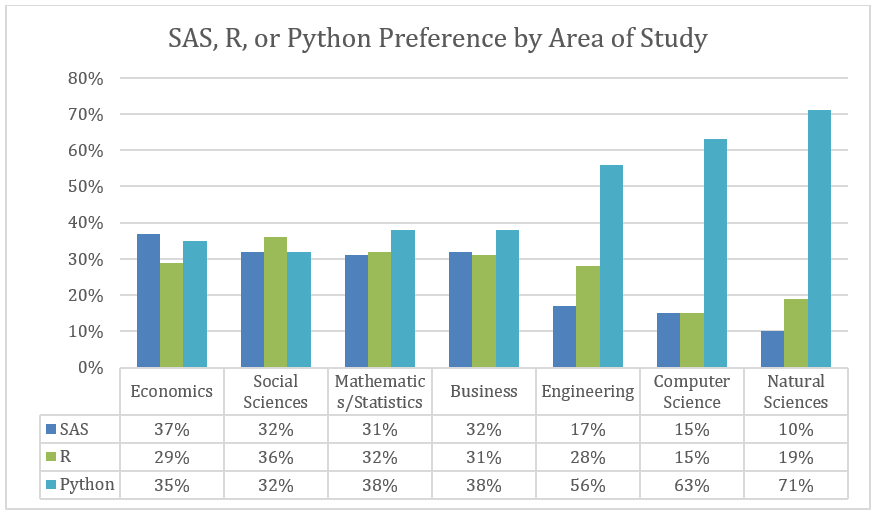
\includegraphics[width=\linewidth]{figures/Ch3/BigDataTools.PNG}
\caption{SAS, R or Python preferences \cite{Siddiqui2015}}
\label{f:soft-preferences}
\end{figure}

\begin{figure}[h]
\centering
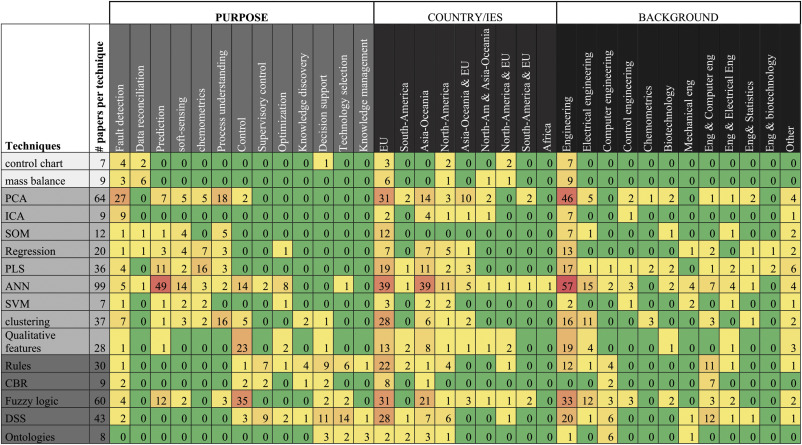
\includegraphics[width=0.9\linewidth]{figures/Ch3/PaperTable.jpg}
\caption{Techniques in WWT  \cite{Corominas2018}.}
\label{f:Papers Table}
\end{figure}

\begin{figure}[h]
\centering
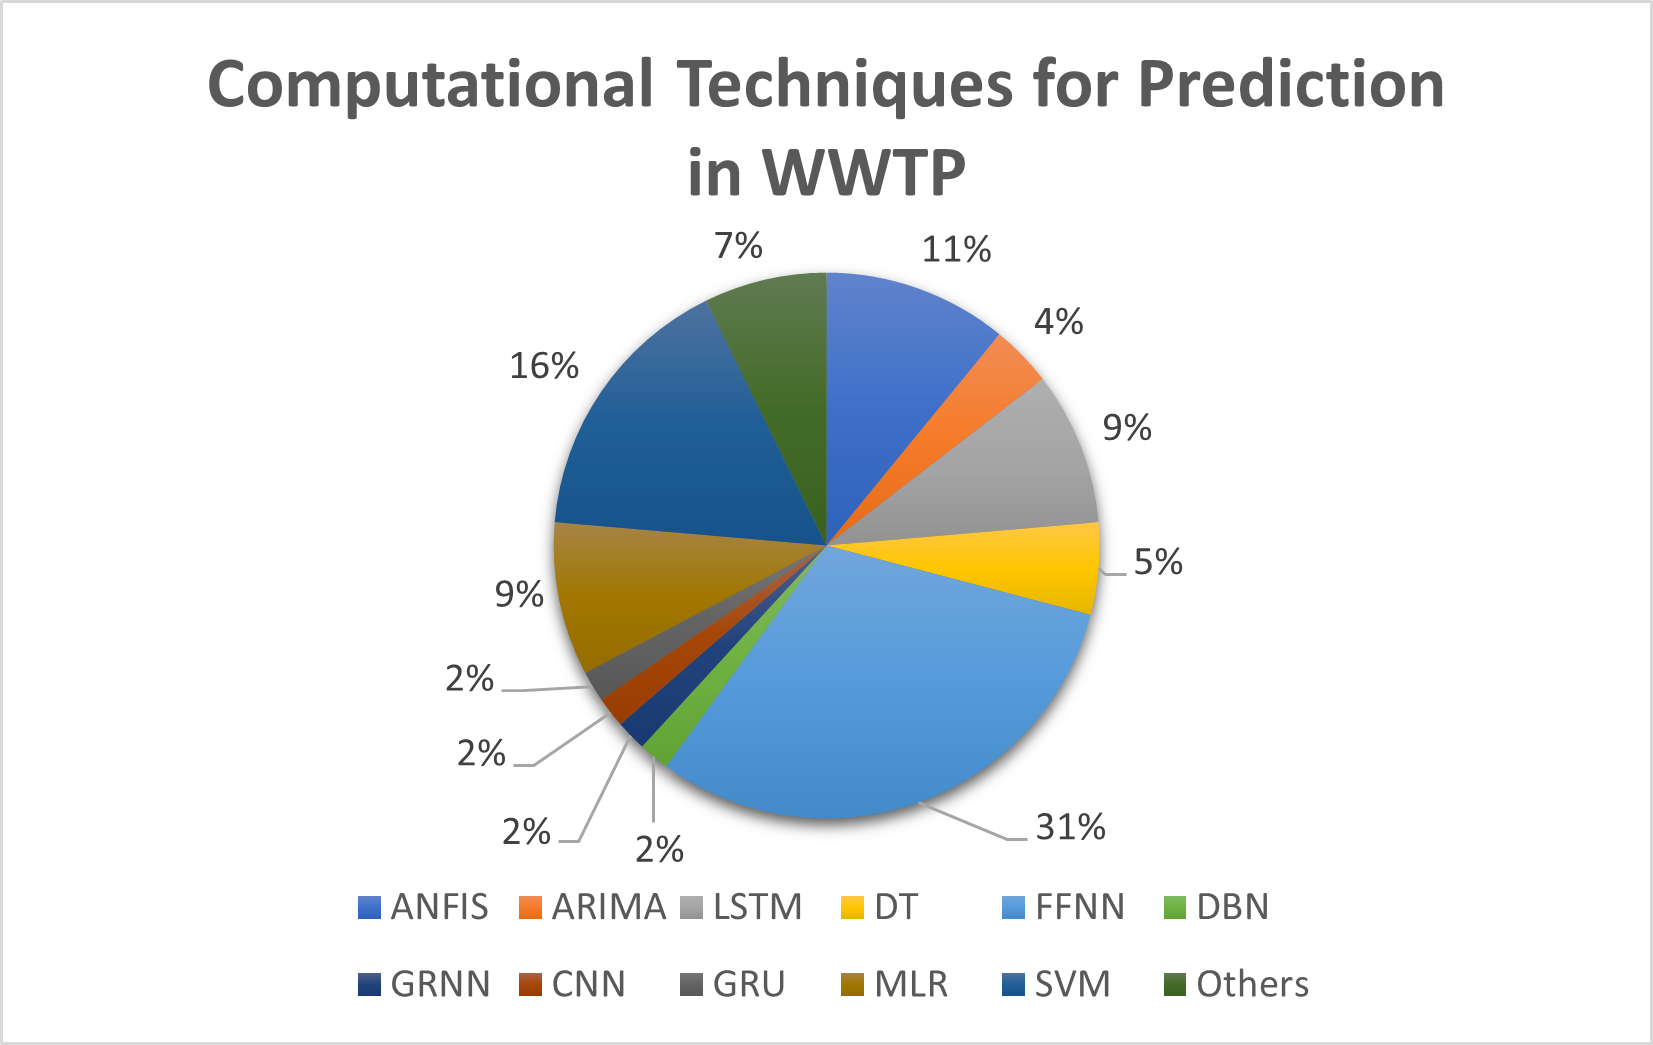
\includegraphics[width=0.8\linewidth]{figures/Ch3/Prediction_model_dist.png}
\caption{Techniques used for Prediction in WWT field}
\label{f:techniques-prediction}
\end{figure}

\autoref{f:Papers Table} presented by \cite{Corominas2018} shows the number of papers per technique used in \ac{WWT}, categorized based on purposes, countries and the authors' background. The search was done in SCOPUS, and the results include papers until 2015, papers published before 2010 and with less than five citations were not included. \autoref{f:techniques-prediction} summarizes the \ac{ML} techniques distribution used for prediction and presented in \autoref{s:RelatedWorks-variablePrediction}. \ac{FFNN}, \ac{ANFIS}, \ac{SVM} are place in the top 3 being the most used ones.
%\section{Summary}
%\label{s:Related-Works-Summary}